\section{Test på LEGO bil}

Gennem projektarbejdet, har gruppen testet den endelige løsning på lego-bilen. Men da simuleringen af det digitale system ikke fungerede, er der kun testet med kontinuere systemblokke. Dette har dog den ulempe, at vi bliver nød til, at samle på systemet, og derfor kommer systemet ikke til at være 100\% perfekt, da vi ikke kan sample uendeligt. Dog burde vores realisering, ligne vores simulering, hvor vi også har indført et integrale led digitalt (altså samplet). \\
Under realiseringen, opdagede vi dog endnu en fejlkilde, som gjorde at systemet opførte sig anderledes. Dette kom af den friktion som systemet har. Denne friktion er nemlig ikke liniær, hvilket betyder, at modstanden falder, når spændingen til motoren når en bestemt størrelse. Derfor får systemet et kraftigt udsving, da den overkompentserer for en fejl. Projektet har derfor et realiseringproblem, og vil skulle bruge en meget hurtig regulerings sløjfe, for at kunne korrigere for fejlen. Dette er nok ikke muligt i praksis, hvorfor en bedre løsning ville være at indføre 2 systemer. Her ville det første system, have control over motoren, når friktionen var belastende, og et system, som tager over når friktionen falder kraftig i belastning. På figur \ref{fig:lego_bil} vises et billede af realiseringen, hvor aksen med hjulene står med en skæv vinkel, mens at aksen med kroppen af bilen, står vandret. 

\begin{figure}[H]
	\centering
	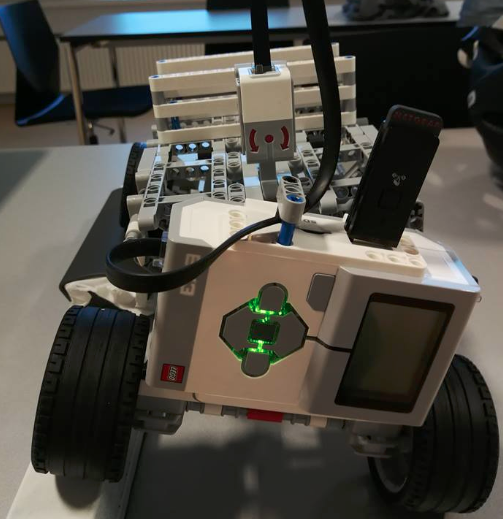
\includegraphics[width = 300pt]{figur/lego_bil}
	\caption{Lego realisering}
	\label{fig:lego_bil}
\end{figure}   